%%%%%%%%%%%%%%%%%%%%%%%%%%%%%%%%%%%%%%%%%%%%%%%%%%%%%%%%%%%%

\section{Explorative study}
\label{S:study}

In this study, we examine some \Wikipedia{} categories with two objectives: a) to retrieve some candidate classifiers of an emerging taxonomy of software languages; b) to get some experience with \Wikipedia's approach to classification and related issues of style and consistency.\footnote{All \Wikipedia{} access for this study was validated (again) during 7-18 June 2013 which is also when quotes were extracted from \Wikipedia, as they appear in the text of this section.}

%%%%%%%%%%%%%%%%%%%%%%%%%%%%%%%%%%%%%%%%%%%%%%%%%%%%%%%%%%%%

\paragraph*{\textbf{Designation of a root}}

\Wikipedia's classification hierarchies are complex and thus, it is not straightforward to determine a root for exploration unambiguously. However, we have established by an ad-hoc search that the category \WikipediaCategory{Computer languages} may be a suitable root as its intended coverage may be similar to what the SL(E) community has in mind for the notion of software languages. 

%%%%%%%%%%%%%%%%%%%%%%%%%%%%%%%%%%%%%%%%%%%%%%%%%%%%%%%%%%%%

\begin{figure}[t!]
\begin{center}
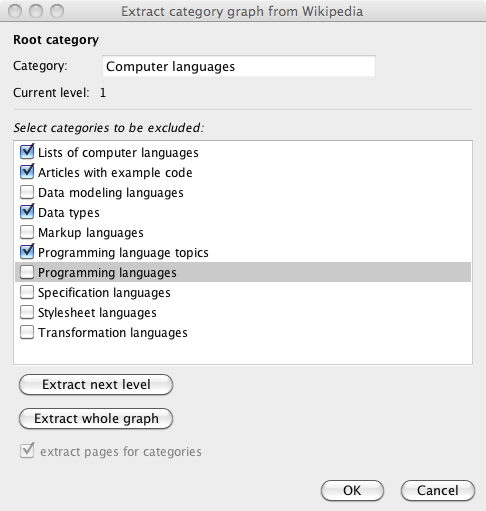
\includegraphics[width=.5\textwidth]{figures/clLevel1.png}
\end{center}
\vspace{-66\in}
\caption{Extraction and reduction of level 1 subcategories for \emph{Computer languages}.}
\label{F:clLevel1}
\vspace{-42\in}
\end{figure}

%%%%%%%%%%%%%%%%%%%%%%%%%%%%%%%%%%%%%%%%%%%%%%%%%%%%%%%%%%%%

Category \WikipediaCategory{Computer languages} only has a few immediate subcategories; see \autoref{F:clLevel1}. The figure shows the situation in the \WikiTax{} dialog past selecting a few level 1 categories for exclusion. That is, \WikipediaCategory{Lists of computer languages}, \WikipediaCategory{Articles with example code}, \WikipediaCategory{Data types}, and \WikipediaCategory{Programming language topics} should be excluded because they are not directly concerned with the \emph{classification} of languages.

We also observe that the category \WikipediaCategory{Programming languages} is reachable in one step from \WikipediaCategory{Computer languages} while there is another major classifier for programming languages, namely \WikipediaCategory{Programming language classification}, which would be reachable through the excluded category \WikipediaCategory{Programming language topics}.

%%%%%%%%%%%%%%%%%%%%%%%%%%%%%%%%%%%%%%%%%%%%%%%%%%%%%%%%%%%%

\begin{figure}[t!]
{\footnotesize

\begin{center}
\noindent
\begin{tabular}{l|p{3.4in}}
\textbf{Category} & \textbf{Subcategories} \\\hline
\input{../data/Computer_languages.tex-twolevels}
\end{tabular}
\end{center}

\vspace{-42\in}

}
\caption{Reduced subcategory lists for subcategories of \emph{Computer languages}.}
\label{F:twolevels}
\vspace{-42\in}
\end{figure}

%%%%%%%%%%%%%%%%%%%%%%%%%%%%%%%%%%%%%%%%%%%%%%%%%%%%%%%%%%%%

\paragraph*{\textbf{Level-by-level extraction}}

We decided to extract another level to obtain a graph of manageable size. Again, we excluded several categories, if they did not meet our objective of language classification. As a result, we obtained the categories shown in \autoref{F:twolevels}. This is a pretty manageable set of language classifiers. 
It happens that they all end on ``... languages'' except for two subcategories of \WikipediaCategory{Markup languages} which end on ``... formats''. In contrast, most of the excluded categories (see below) do not end on ``... languages'' . We take this to provide a hint at the different classification styles of \Wikipedia.

%%%%%%%%%%%%%%%%%%%%%%%%%%%%%%%%%%%%%%%%%%%%%%%%%%%%%%%%%%%%

\begin{figure}[t!]
{\footnotesize

\begin{center}
\noindent
\begin{tabular}{l|l}
\textbf{Category} & \textbf{Meta classifier} \\\hline
\input{../data/Computer_languages.tex-metaclassify}
\end{tabular}
\end{center}

\vspace{-42\in}

}
\caption{Exclusion summary for levels 1 and 2 of \emph{Computer languages}; this list is produced by the \WikiTax{} tool based on metadata (comments) entered by us interactively.}
\label{F:metaclassify}
\vspace{-42\in}
\end{figure}

%%%%%%%%%%%%%%%%%%%%%%%%%%%%%%%%%%%%%%%%%%%%%%%%%%%%%%%%%%%%

\paragraph*{\textbf{Classifier classification}}

In order to obtain the reduced result of \autoref{F:twolevels}, we had to exclude 29 categories. This may seem like a small number, but it is clear that we will need to exclude much more categories once we push extraction deeper into the category graph. Thus, we embarked on the classification of reasons for exclusion, thereby standardizing comments for exclusion, also suggesting a foundation for reproducing our results. We identified the following classifiers; see \autoref{F:metaclassify} for the full list of excluded categories with the associated classifier:

\smallskip

{\small

\begin{description}

\item[Alternative classifier] The category classifies software languages in a manner that is not related to software concepts. For instance, the category \WikipediaCategory{Academic programming languages} describes itself as being concerned with languages that are ``influential in computer science and programming language theory''.

\item[Deviating classifier] The category does not actually classify software languages. It rather classifies something else. For instance, category \WikipediaCategory{Articles with example code} describes itself as being concerned with ``articles which include reference implementations of algorithms''.

\item[Singleton classifier] The category is effectively concerned with a single software language for which it serves as a container of related entities such as technologies or standards. For instance, category \WikipediaCategory{Cascading Style Sheets} contains pages on all kinds of topics related to the CSS language.

\item[List classifier] The category collects lists or categories of lists (rather than plain categories) of software languages. For instance, category \WikipediaCategory{Lists of computer languages} has \WikipediaCategory{Lists of programming languages} as a subcategory, which in turn contains pages for some lists of languages, such as the \WikipediaPage{List of BASIC dialects}.

\item[Maintenance classifier] The category is used by the \Wikipedia{} authors to capture some information related to the maintenance of content. For instance, category \WikipediaCategory{Markup language stubs} describes itself as serving ``for stub articles relating to markup languages''.

\end{description}

}

%%%%%%%%%%%%%%%%%%%%%%%%%%%%%%%%%%%%%%%%%%%%%%%%%%%%%%%%%%%%

\paragraph*{\textbf{An observation regarding \Wikipedia{} style}}

At this point, exploration already had led to a manageable view on the category graph for software languages. This view is, in fact, quite effective, which we illustrate with an inquiry that suggested itself during exploration.

Looking at \autoref{F:clLevel1} and \autoref{F:twolevels}, we may suspect an asymmetry between `query' versus `transformation'. That is, there is a category \WikipediaCategory{Transformation languages} at level 1, but there is apparently no category for `query languages', not even at level 2. Let us inspect the page for \WikipediaPage{SQL}, which is arguably a quite obvious query language. It turns out that \WikipediaPage{SQL} is a member of various categories including a category \WikipediaCategory{Query languages} which in turn is subcategory of various categories including the category \WikipediaCategory{Domain-specific programming languages} which occurred in \autoref{F:twolevels}. Let us compare this classification scheme with the one of \WikipediaPage{XSLT}, which is arguably a quite obvious transformation language: it is a member of the categories \WikipediaCategory{Transformation languages}, \WikipediaCategory{Declarative programming languages}, \WikipediaCategory{Functional languages}, \WikipediaCategory{Markup languages}, \WikipediaCategory{XML-based programming languages}, and yet other categories that may count as `alternative classifiers'. However, \WikipediaPage{XSLT} (unlike \WikipediaPage{SQL}) is not a member of the category \WikipediaCategory{Domain-specific programming languages}.

We take this sort of observation to mean that the derivation of a highly consistent taxonomy for software languages would require some non-trivial effort in defining and enforcing principles. We were not able to observe this situation so clearly prior to using \WikiTax.

%%%%%%%%%%%%%%%%%%%%%%%%%%%%%%%%%%%%%%%%%%%%%%%%%%%%%%%%%%%%

\paragraph*{\textbf{ Programming languages: all levels}}

\autoref{F:twolevels} makes it obvious that the subcategory of \WikipediaCategory{Computer languages} with by far the most subcategories is 
\WikipediaCategory{Programming languages}. Thus, we embarked on a more comprehensive exploration of category \WikipediaCategory{Programming languages}:

%%%%%%%%%%%%%%%%%%%%%%%%%%%%%%%%%%%%%%%%%%%%%%%%%%%%%%%%%%%%

\begin{figure}[t!]
\parbox{.48\textwidth}{
Pages

\noindent 
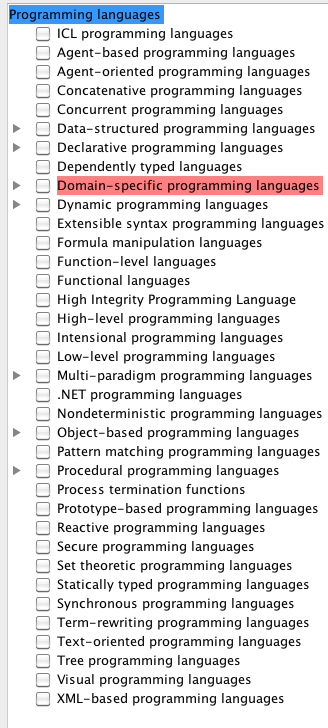
\includegraphics[width=0.41\textwidth]{figures/plPagesTransitive.png}
}\hfill\parbox{.48\textwidth}{

Categories 

\noindent 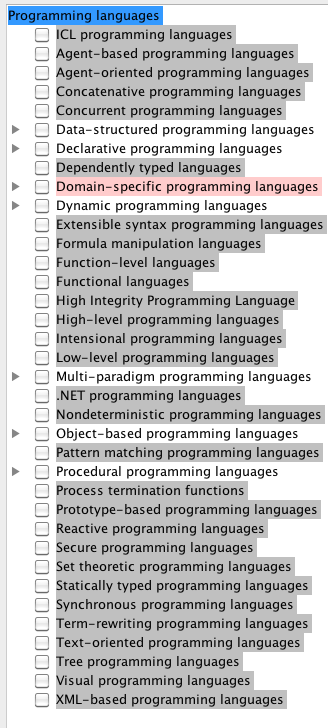
\includegraphics[width=0.41\textwidth]{figures/plSubcategoriesTransitive.png}
}

\vspace{-42\in}

\caption{Metrics-based views on \emph{Programming languages} graph.}
\label{F:plNumbers}
\vspace{-42\in}
\end{figure}

%%%%%%%%%%%%%%%%%%%%%%%%%%%%%%%%%%%%%%%%%%%%%%%%%%%%%%%%%%%%

Initially, we extracted 423 categories over 8 levels with 7515 pages. The automatic extraction took several minutes. We performed exclusion in two steps. First, we excluded direct subcategories of the category \WikipediaCategory{Programming languages}---based on the list in \autoref{F:metaclassify}. After such initial pruning, 288 categories with 6671 pages remained. We completed reduction at all levels of the category graph. This process required about 2 hours of manual work---work that is mainly concerned with checking assumptions for exclusion by consulting corresponding category pages on \Wikipedia. Ultimately, 79 categories over 4 levels with 1560 pages remained.  \autoref{F:plNumbers} visualizes the reduced taxonomy while applying two different metrics, as supported by \WikiTax.

On the left, the metric for the \emph{number of transitive member pages} is applied for visualization. No category is grayed out, which means that there is no category without members. Most of the categories are shown in a plain font, which means that they all carry members, but less than 25\,\% of the total members in the category \WikipediaCategory{Programming languages} (which has 1560 member pages). There is actually one heavyweight: category \WikipediaCategory{Domain-specific programming languages} carries 976 members, which is more than 50\,\% of all members; this status is expressed by 
highlighting the category.

On the right, the metric for the number of transitive subcategories is applied for visualization. Most subcategories of \WikipediaCategory{Programming languages} do not have any subcategories; thus, they are grayed out. 7 out of 36 level-1 categories carry subcategories. 6 out of these 7 categories carry only very few subcategories (less than 5). Category \WikipediaCategory{Domain-specific programming languages} carries 18 subcategories, which is more than 25\,\% of all subcategories; this status is expressed by highlighting the category.

%%%%%%%%%%%%%%%%%%%%%%%%%%%%%%%%%%%%%%%%%%%%%%%%%%%%%%%%%%%%
